\documentclass[12pt,graphicx,caption,rotating]{article}
\textheight=23cm
\textwidth=17cm
\topmargin=-1cm
\oddsidemargin=0cm
\usepackage[activeacute,spanish]{babel}
\usepackage[utf8]{inputenc}
\usepackage{graphicx}%manejo de graficos
\usepackage{times}
\usepackage{amssymb,amsfonts}
\usepackage[tbtags]{amsmath}
\usepackage{cite}
\usepackage[all]{xy}
\usepackage{subfigure}
\usepackage{wrapfig}
\usepackage{color}
\usepackage{multicol}
\usepackage{cite}
\usepackage{url}
\usepackage[tbtags]{amsmath}
\usepackage{amsmath,amssymb,amsfonts,amsbsy}
\usepackage{bm}
\usepackage{algorithm}
\usepackage{algorithmic}
\usepackage[all]{xy}
\usepackage[centerlast, small]{caption}
\usepackage[colorlinks=true, citecolor=blue, linkcolor=blue, urlcolor=blue, breaklinks=true]{hyperref}
\hyphenation{ele-men-tos he-rra-mi-en-ta cons-tru-yen trans-fe-ren-ci-a pro-pu-es-tas si-mu-lar vi-sua-li-za-cion}

\begin{document}
\begin{titlepage}
\begin{center}
{\huge \textbf{Implememtacion de la herramienta PinaVM ayudada por SystemC}}\\[5cm]
{\Large \textbf{Integrantes:}}\\
{\Large David Ricardo Martínez Hernandez Código: $214997$}\\
{\Large Sergio Ándres Zapata Palomino Código: $261261$}\\[5cm]
{\Large \textbf{Verificación de Sistemas Digitales}}\\
{\Large Johan Sebastian Eslava Grazón}\\
{\Large José Alejandro Duque Rueda}\\[6cm]
{\Large Universidad Nacional de Colombia}\\
{\Large Facultad de Ingeniería}\\
{\Large Bogotá}\\
\date{}
\end{center}
\end{titlepage}

\floatname{algorithm}{Algoritmo}

\section{Que es PinaVM}
\noindent
PinaVM es una herramienta que sirve como Front-end a System C, está basado en LLVM (Low Level Virtual Machine), fue desarrollado a partir de la herramienta PINAPA, otro front-end de System C que actualmente se encuentra descontinuado. PinaVM permite obtener una representación abstracta de un programa hecho en System C.\\
Pinapa es la predecesora de PinaVM, a diferencia de esta última no está basada en LLVM sino en GCC, lo que lo puso en ventaja con respecto a otros intentos de front-end para System C. Sin embargo presentaba varios problemas en su flujo de datos (GCC CFG) además de que el hecho de basarse en GCC dificultaba su instalación y compilación  por lo que finalmente fue reemplazado por PinaVM.

\subsection{Descarga de PinaVM}
\noindent
Para descargar PinaVM se puede hacer desde la consola con los siguiente pasos:
\begin{enumerate}
 \item Abra la terminal o haga lo siguiente $Ctrl \, T$.
 \item Dirijase a la carpeta en donde quiere descargar el repositorio por ejemplo\\ \textbf{\textit{cd Documents/Verificacion/}}
 \item Escribe el siguiente comando en consola\\ \textbf{\textit{git clone https://forge.imag.fr/anonscm/git/pinavm/pinavm.git}}
\end{enumerate}
\noindent
Al realizar esta labor se crea una carpeta con el nombre de PinaVM.

\section{Instalación de Requerimientos}
\noindent
Algunas de las herramientas que son pre-requisito para poder utilizar PinaVM ya han sido previamente instaladas porque han sido utilizadas en cursos anteriores. Esta herramientas son:
\begin{itemize}
 \item GCC: Es un compilador de código abierto.
 \item Cmake: Es un sistema de generación de código abierto multiplataforma.
 \item LLVM: Es un tipo de infraestructura para un compilador y es la herramienta que ayuda a recibir los datos por parte del el Front–end, en este caso PinaVM. En la siguiente Figura~\ref{fig1} se puede ver un esquema de como trabaja el LLVM
 \begin{figure} [H]
 \center
  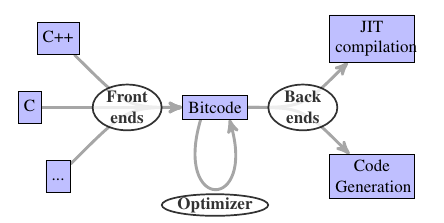
\includegraphics[scale=0.5]{llvm.png}
  \caption{Esquema de trabajo del LLVM (Tomado de \cite{page2})}
  \label{fig1}
 \end{figure}
 \item Clang: Clang es un compilador para $C / C + +$ basado en LLVM.
\end{itemize}

\subsection{GCC}
\noindent
PinvaVM requiere la versión que se encuentre disponible en su sistema operativo, si no lo tiene instala siga los siguientes pasos:
\begin{enumerate}
 \item Abra la terminal o haga lo siguiente $Ctrl \, T$.
 \item Escriba en la consola \textbf{\textit{sudo apt-get install gcc}}, o si desea alguna versión en particular para otras aplicaciones escriba en la consola \textbf{\textit{sudo apt-get install gcc-X.X}}, donde $X.X$ es la versión que desea
\end{enumerate}

\subsection{Cmake}
\noindent
Para ejecutar PinaVM requiere la versión más reciente de Cmake, se  puede uditilizar desde la versión $2.8.8$, o dirigirse a la página \url{http://www.cmake.org/cmake/resources/software.html} y descargar la versión $2.12.8.1$. Después de haber descargado el archivo haga lo siguiente:
\begin{itemize}
 \item Abra la terminal o haga lo siguiente $Ctrl \, T$.
 \item Diríjase a la carpeta en donde descargo el archivo, generalmente se encuentra en la carpeta Downloads con el comando \textbf{\textit{cd Downloads}} 
 \item Luego ejecute el siguiente comando \textbf{\textit{tar zxvf nombre\_archivo.tar.gz}} 
 \item Luego se dirigen a la carpeta \textbf{\textit{cmake-2.X.8.X}} con el comando \textbf{\textit{cd cmake-2.X.8.X}} 
 \item Ejecutan el siguiente comando \textbf{\textit{sudo ./configure}} .
 \item Después \textbf{\textit{sudo ./bootstrap}} 
 \item Ya casi para finalizar ejecutan \textbf{\textit{sudo make}} 
 \item Y finalmente \textbf{\textit{sudo make install}} 
\end{itemize}

\subsection{LLVM}
\noindent
La versión mínima del LLVM que requiere PinaVM es la $3.2$, existen varias formas de instalarla. Si tiene la distribución de Ubuntu $12.04$ haga lo siguiente:
\begin{enumerate}
 \item Abra la terminal o haga lo siguiente $Ctrl \, T$.
 \item Escriba en la consola \textbf{\textit{sudo apt-get install llvm}} , luego actualiza a la versión $3.2$ o $3.3$ según desee, con el comando\\ \textbf{\textit{sudo apt-get install llvm-3.X llvm-3.X-dev llvm-3.X-examples llvm-3.X-runtime}} 
\end{enumerate}
\noindent
O se puede realizar instalación desde el código fuente:
\begin{enumerate}
 \item Primero se debe descargar el archivo \textit{llvm-3.4.src.tar.gz} que se encuentra en la página \url{http://llvm.org/releases/download.html#3.4}.
 \item Abra la terminal o haga lo siguiente $Ctrl \, T$.
 \item Diríjase	 a la carpeta en donde descargo el archivo, generalmente es en Downloads, por ejemplo \textbf{\textit{cd Downloads}}
 \item Luego ejecute el siguiente comando \textbf{\textit{tar zxvf llvm-3.4.src.tar.gz}} 
 \item ingrise a la carpeta que se creo \textbf{\textit{cd llvm-3.4}}
 \item Luego ejecute el comando \textbf{\textit{sudo ./configure}}
 \item Después ejecute el comando \textbf{\textit{sudo make}}
 \item Y finalmente ejecute el comando \textbf{\textit{sudo make install}}
\end{enumerate}

\subsection{Clang}
\noindent
La versión necesaria de Clang para ejecutar PinaVM es la $3.2$, Ubuntu $12.04$ tiene en sus repositorios la versión $3.3$, se puede instalar de la siguiente forma:
\begin{enumerate}
 \item Abra la terminal o haga lo siguiente $Ctrl \, T$.
 \item Escriba en la consola \textbf{\textit{sudo apt-get install clang}} , luego escriba lo siguiente \textbf{\textit{sudo apt-get install clang-3.3 clang-format-3.3}} 
\end{enumerate}

\section{Instalación de PinaVM}
\noindent
Al haber realizado las instalaciones previas se puede continuar con la instalación de PinaVM. Siguiendo los siguientes pasos:
\begin{enumerate}
 \item Entrar a la carpeta donde quiere realizar la instalación de PinaVM por ejemplo\\
	\textbf{\textit{cd Documents/Verificacion/Proyecto}}
 \item Al ingresar a dicha carpeta se ejecuta lo siguiente:
 \begin{itemize}
  \item ckmake /carpeta\_PinaVM/, para el caso de ejemplo seria\\
  \textbf{\textit{cmake /home/usuario/Documents/Verificacion/PinaVM}}
 \end{itemize}
 \item Finalmente se ejecuta el comando \textbf{\textit{sudo make}}
\end{enumerate}
\noindent
\textcolor{red}{Nota:} Si aparece el error:
 \begin{verbatim}
  /home/user_name/../PinaVM/backends/PromelaBackend
  /PromelaBackend.cpp:23:29: fatal error: llvm/DataLayout.h: No such file
  or directory compilation terminated.
  make[2]: *** [backends/PromelaBackend/CMakeFiles/promela.dir/
  PromelaBackend.cpp.o]
  Error 1
  make[1]: *** [backends/PromelaBackend/CMakeFiles/promela.dir/all]
  Error 2
  make: *** [all] Error 2
 \end{verbatim}
La solución que se debe hacer es copiar o generar un enlace de la librería. utilizando el siguiente comando \textbf{\textit{locate llvm/DataLayout.h}}, generalmente saldrá \textbf{\textit{/usr/include/llvm-3.2/llvm/DataLayout.h}}, entonces cree un directorio nuevo en \textbf{\textit{/usr/include}} llamado llvm en vez de \textbf{\textit{llvm-3.2}} y o copia todos los archivos o haga enlaces simbólicos.\\\\
Si al realizar el procedimiento anterior no sale ningún error en la consola, PinaVM quedo instalado en el computador.

\bibliographystyle{ieeetran}
\begin{thebibliography}{99}

\bibitem{page1} Main Page to the project PinaVM. Sitio web ``\url{https://forge.imag.fr/plugins/mediawiki/wiki/pinavm/index.php/Main_Page}'', visitada el 20 de Enero de 2014.

\bibitem{page2} Marquet, Kevin and Moy, Matthieu. PinaVM: a SystemC Front-End Based on an Executable Intermediate Representation. Abril de 2012. Sitio web ``\url{http://www-verimag.imag.fr/TR/TR-2010-8.pdf}'', visitada el 20 de Enero de 2014.

%\bibitem{page3} Impatt Diode. Sitio web ``\url{http://en.wikipedia.org/wiki/Impatt_diode}'', visitada el 20 de Enero de 2014.
\end{thebibliography}
\end{document}